\chapter{Cartographie automatisée d'images aériennes}
	\citationChap{}{}
	\minitoc
	\newpage

%%%%%%%%%%%%%%%%%%%%%%%%%%%%%%%%%%%%%%%%%%%%%%%%%%%%%%%%%%%%%%%%%%%%%%%%%%%%%%%%%%%%%%%%%%%%%

\section{Méthodes de cartographie d'images de télédétection}

Il est possible de distinguer deux étapes dans le processus de classification de données. La première étape, dite d'extraction de caractéristiques, consiste à transformer la donnée pour la projeter dans un espace de représentation adapté. La seconde consiste à la classification à proprement parler, c'est-à-dire à la séparation de l'espace ainsi formé en sous-ensemble disjoints.

Par exemple, dans le cas d'une machine à vecteur de support linéaire, la classification s'effectue en déterminant les hyperplans permettant de séparer au mieux les données. L'espace de représentation doit donc être, si possible, linéairement séparable. Il s'agit alors de trouver des caractéristiques (c'est-à-dire une projection) adaptées.

\subsection{Classification pixelliques}

Une acquisition d'observation de la Terre est caractérisée par sa résolution spatiale. Celle-ci détermine l'unité de surface minimale au sein laquelle il devient impossible de séparer deux observations. Dans le cas d'une image, on exprime généralement la résolution en unité de longueur par pixel. Une image à résolution de 10m/px est un ensemble d'observations, chacune effectuée sur une surface de $10\times10$m.

De fait, en traitement d'images de télédétection, le pixel est l'unité atomique de surface. Par conséquent, une mesure pour 1 pixel est la mesure la plus pure disponible. Sans toutefois prétendre qu'une observation sur un pixel ne souffre pas de problèmes de mélanges (en fonction des objets d'intérêt, un pixel peut mélanger plusieurs classes hétérogènes), le pixel représente la mesure la plus fine disponible.

Par conséquent, en première approche, il semble raisonnable de traiter le problème de cartographie comme un problème de classification des pixels. Il s'agit ainsi de donner à chaque pixel une information sémantique, c'est-à-dire une classe.

Pour ce faire, il est dans un premier temps nécessaire d'extraire des attributs du pixel. Dans le cas d'une image multispectrale, cela peut par exemple être la proportion de lumière réfléchie dans chacune des longueurs d'onde mesurées. Mais il est également possible d'y ajouter d'autres attributs : la valeur moyenne de l'intensité lumineuse ou les observations voisines.

Une fois l'extraction d'attributs effectuée, il est possible de réaliser une classification.

L'avantage de cette méthode est qu'elle garantit une résolution identique à celle de la donnée.

Néanmoins, elle possède deux inconvénients notables. Le premier est que le nombre de pixels devient rapidement très grand à mesure que la résolution spatiale s'améliore et que la taille de l'image augmente. Le problème de classification peut alors devenir intraitable sur ces images, alors que les capteurs tendent justement à s'améliorer en résolution.

Le second inconvénient est que cette méthode est particulièrement susceptible au bruit. En effet, la classification s'effectuant pixel à pixel, la nature des pixels voisins n'est pas forcément prise en compte. Toutefois, les objets géographiques considérés s'étendent bien souvent sur plusieurs pixels et possèdent des propriétés géométriques particulières de connexité et de convexité. Ainsi, un pixel particulier soumis à un bruit extrême (suite à une défaillance du capteur ou à un matériau particulier), celui risque d'être mal classé de manière isolée, alors que son appartenance à une région particulière aurait pu permettre de contourner cette erreur en se basant sur des critères d'homogénéité. Ainsi la classification pixellique tend à produire des cartes exhibant un comportement de bruit poivre-et-sel.

\subsection{Classification par région}

Si la considération de la grille de pixels comme base de découpage d'une image semble naturelle, il est possible d'envisager d'autres découpages.

En particulier, il est envisageable de regrouper des pixels similaires dans des régions homogènes. La similarité peut alors uniquement se fonder sur des critères statistiques liées aux valeurs des pixels, ou à des critères sémantiques. Dans le premier cas, on parlera de "superpixels" et dans le second cas de "segmentation".

De nombreux algorithmes ont été proposés à ces fins, aussi bien dans la communauté télédétection que dans la communauté vision par ordinateur.

Soit segmentation "objet" : Felzenswalb, eCognition
Soit segmentation "superpixels": SLIC, Quickshift

\begin{figure}

\begin{subfigure}{\textwidth}
\begin{subfigure}{0.25\textwidth}
    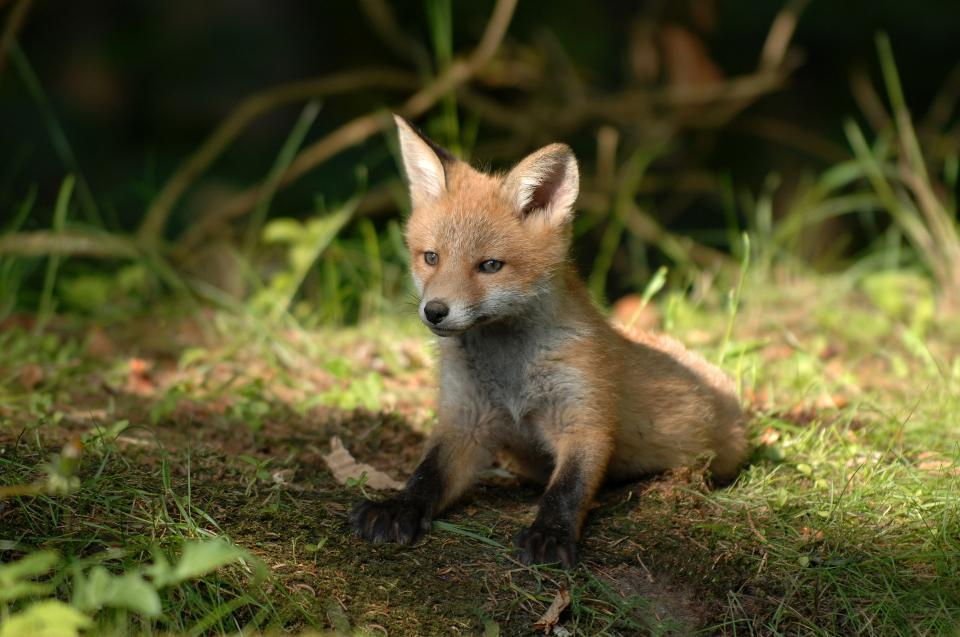
\includegraphics[width=\textwidth]{Chapitre2/fox}
    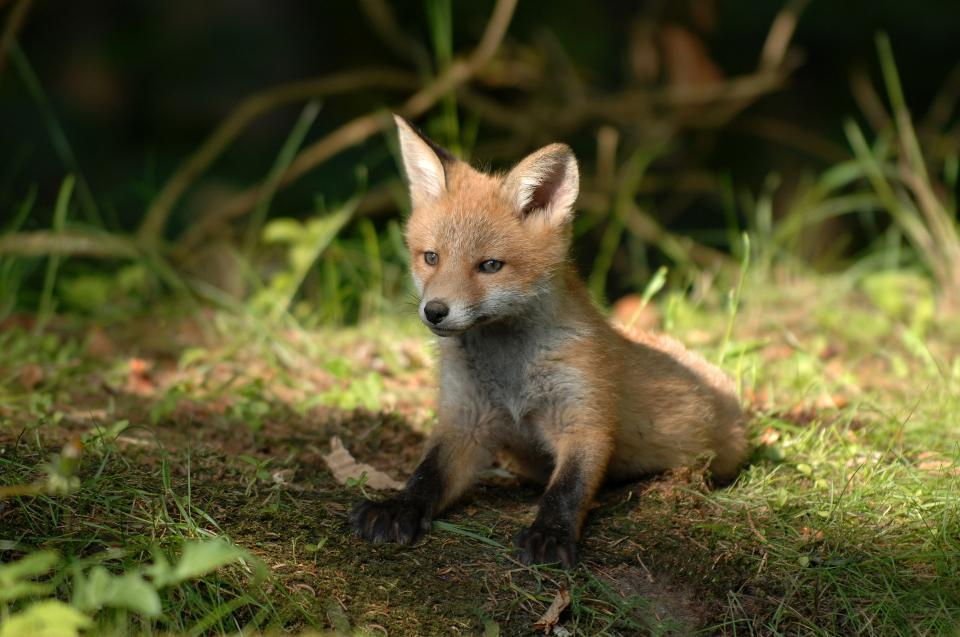
\includegraphics[width=\textwidth]{Chapitre2/fox}
    \caption*{Image originale}
\end{subfigure}%
\begin{subfigure}{0.25\textwidth}
    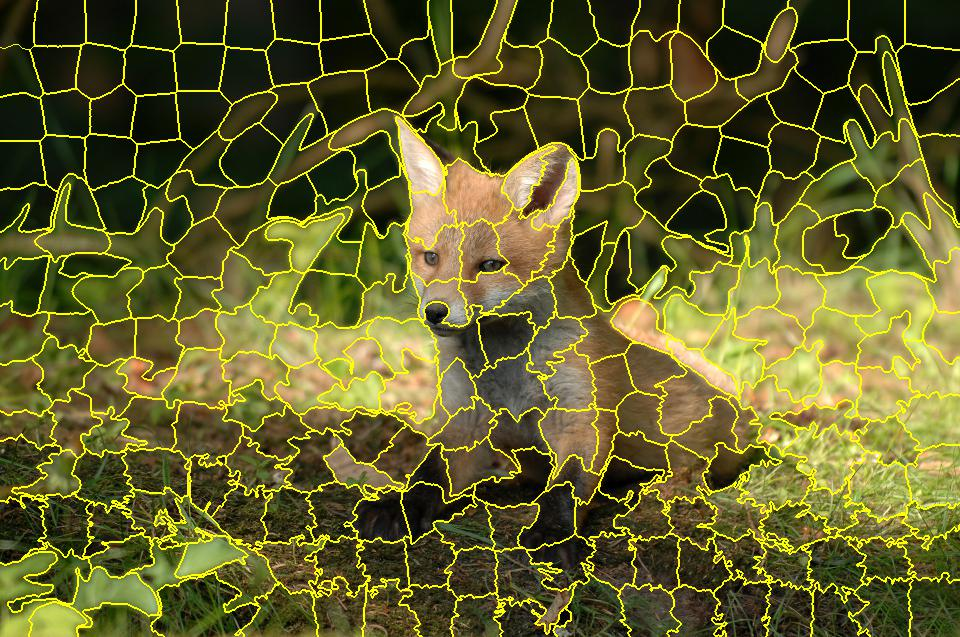
\includegraphics[width=\textwidth]{Chapitre2/fox_slic}
    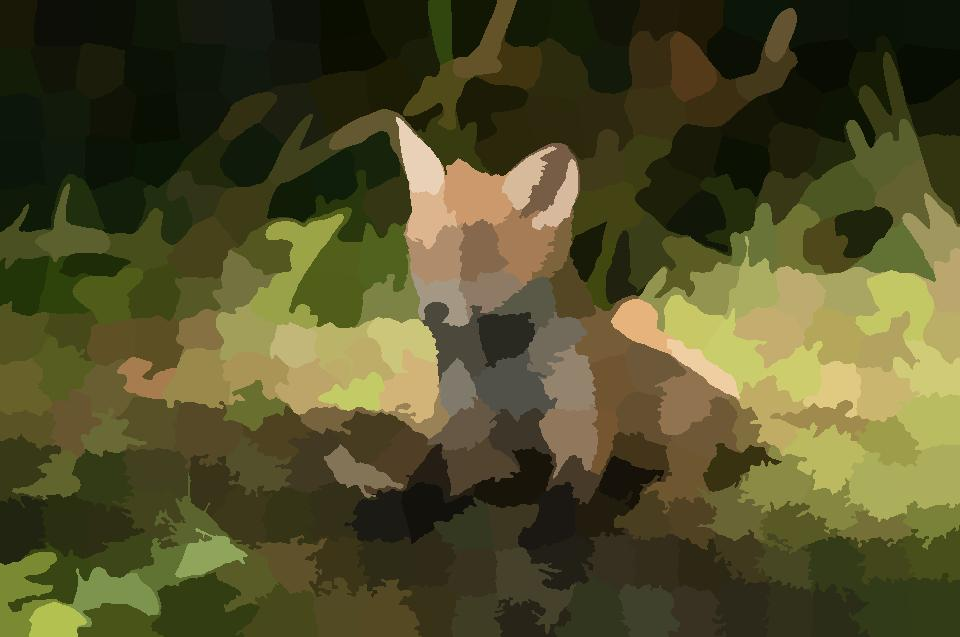
\includegraphics[width=\textwidth]{Chapitre2/fox_slic_patchwork}
    \caption*{SLIC}
\end{subfigure}%
\begin{subfigure}{0.25\textwidth}
    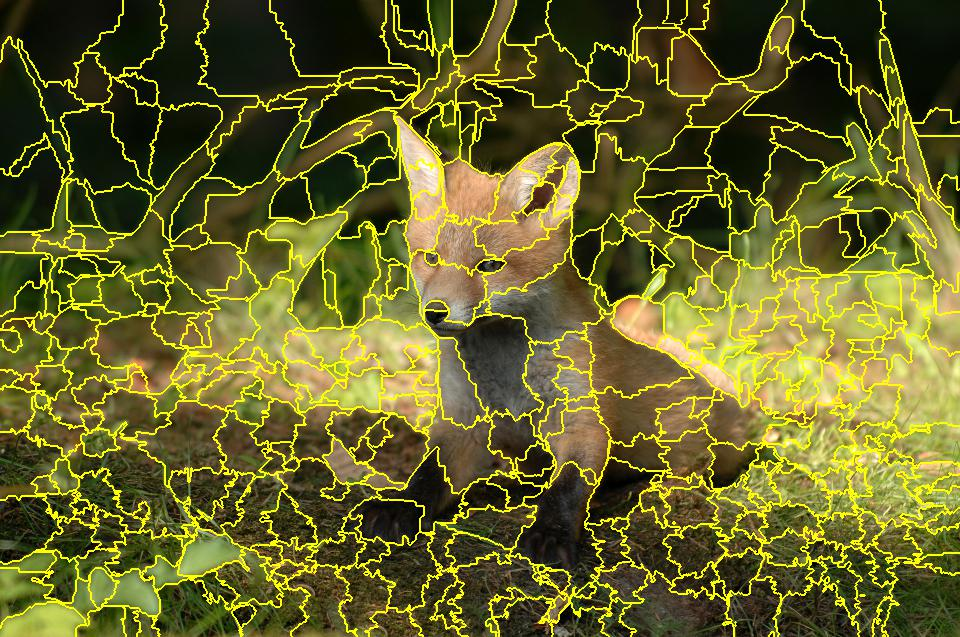
\includegraphics[width=\textwidth]{Chapitre2/fox_quickshift}
    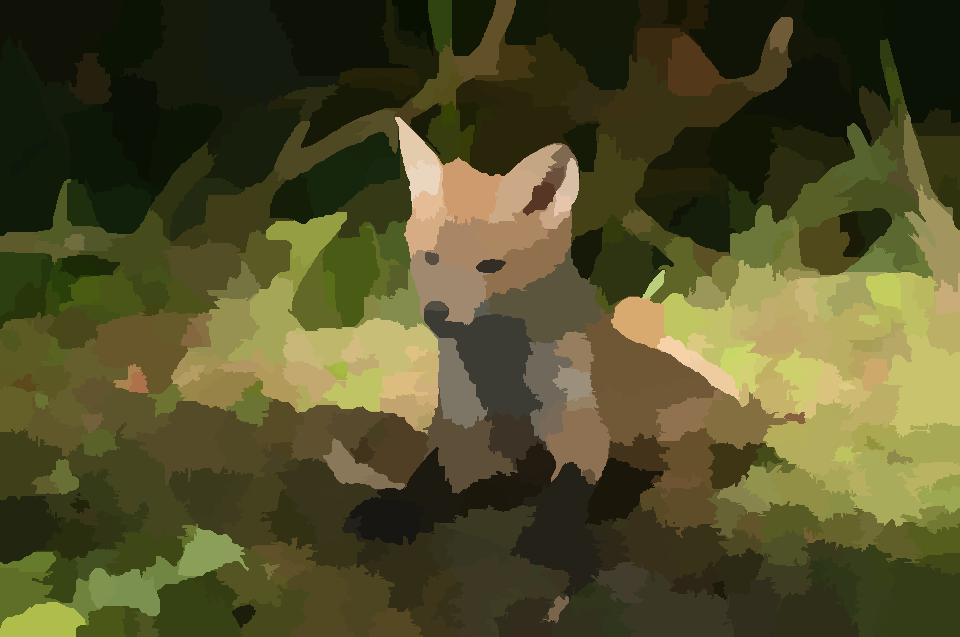
\includegraphics[width=\textwidth]{Chapitre2/fox_quickshift_patchwork}
    \caption*{Quickshift}
\end{subfigure}%
\begin{subfigure}{0.25\textwidth}
    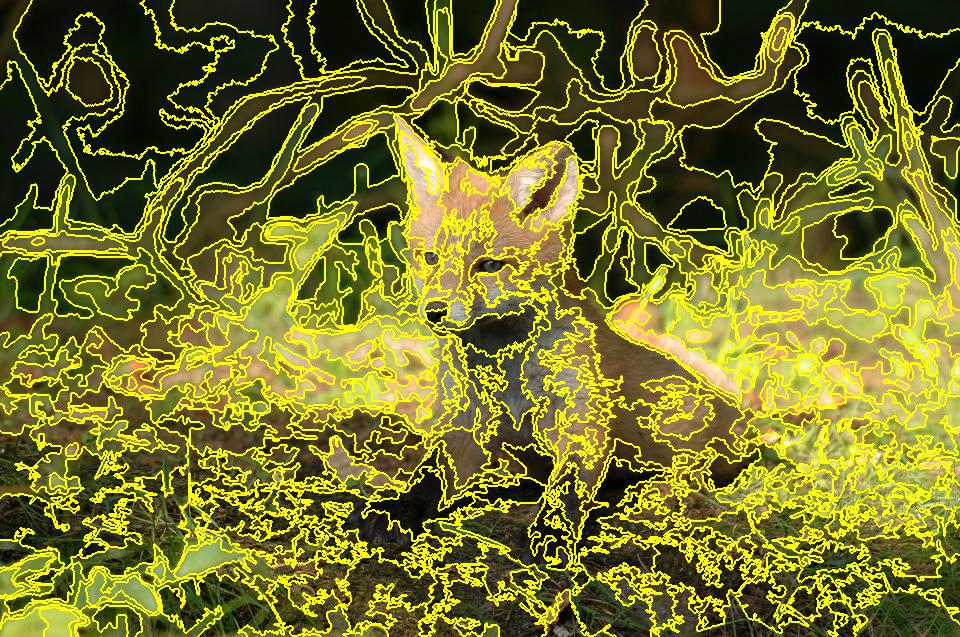
\includegraphics[width=\textwidth]{Chapitre2/fox_ecognition}
    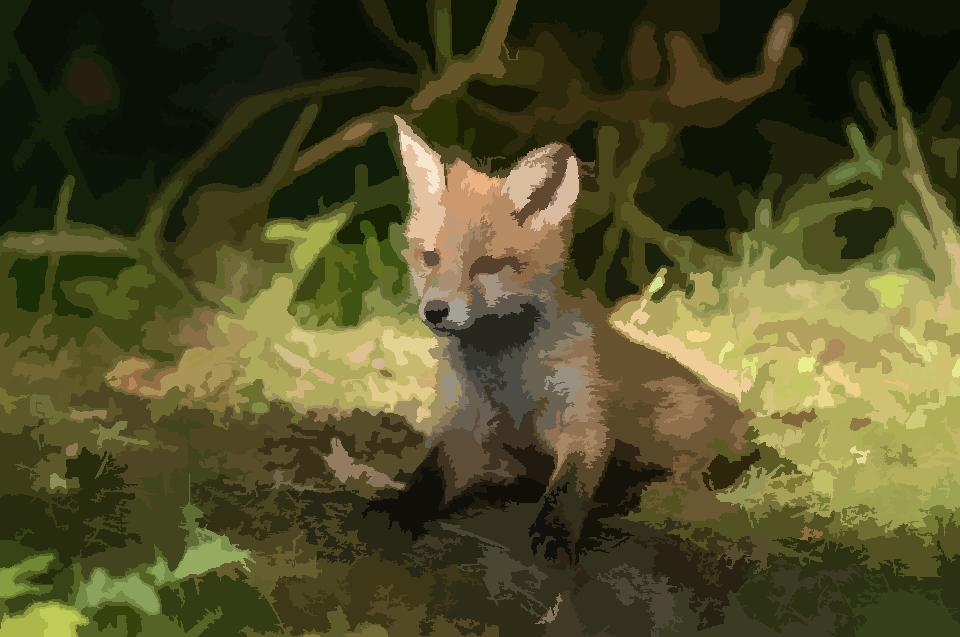
\includegraphics[width=\textwidth]{Chapitre2/fox_ecognition_patchwork}
    \caption*{Algorithme MRS}
\end{subfigure}
\caption{Segmentations d'une image naturelle. Certains algorithmes produisent des régions faiblement régulières, mais capturant mieux les détails de l'image.}
\label{fig:fox_segmentation}
\end{subfigure}

\begin{subfigure}{\textwidth}
\begin{subfigure}{0.25\textwidth}
    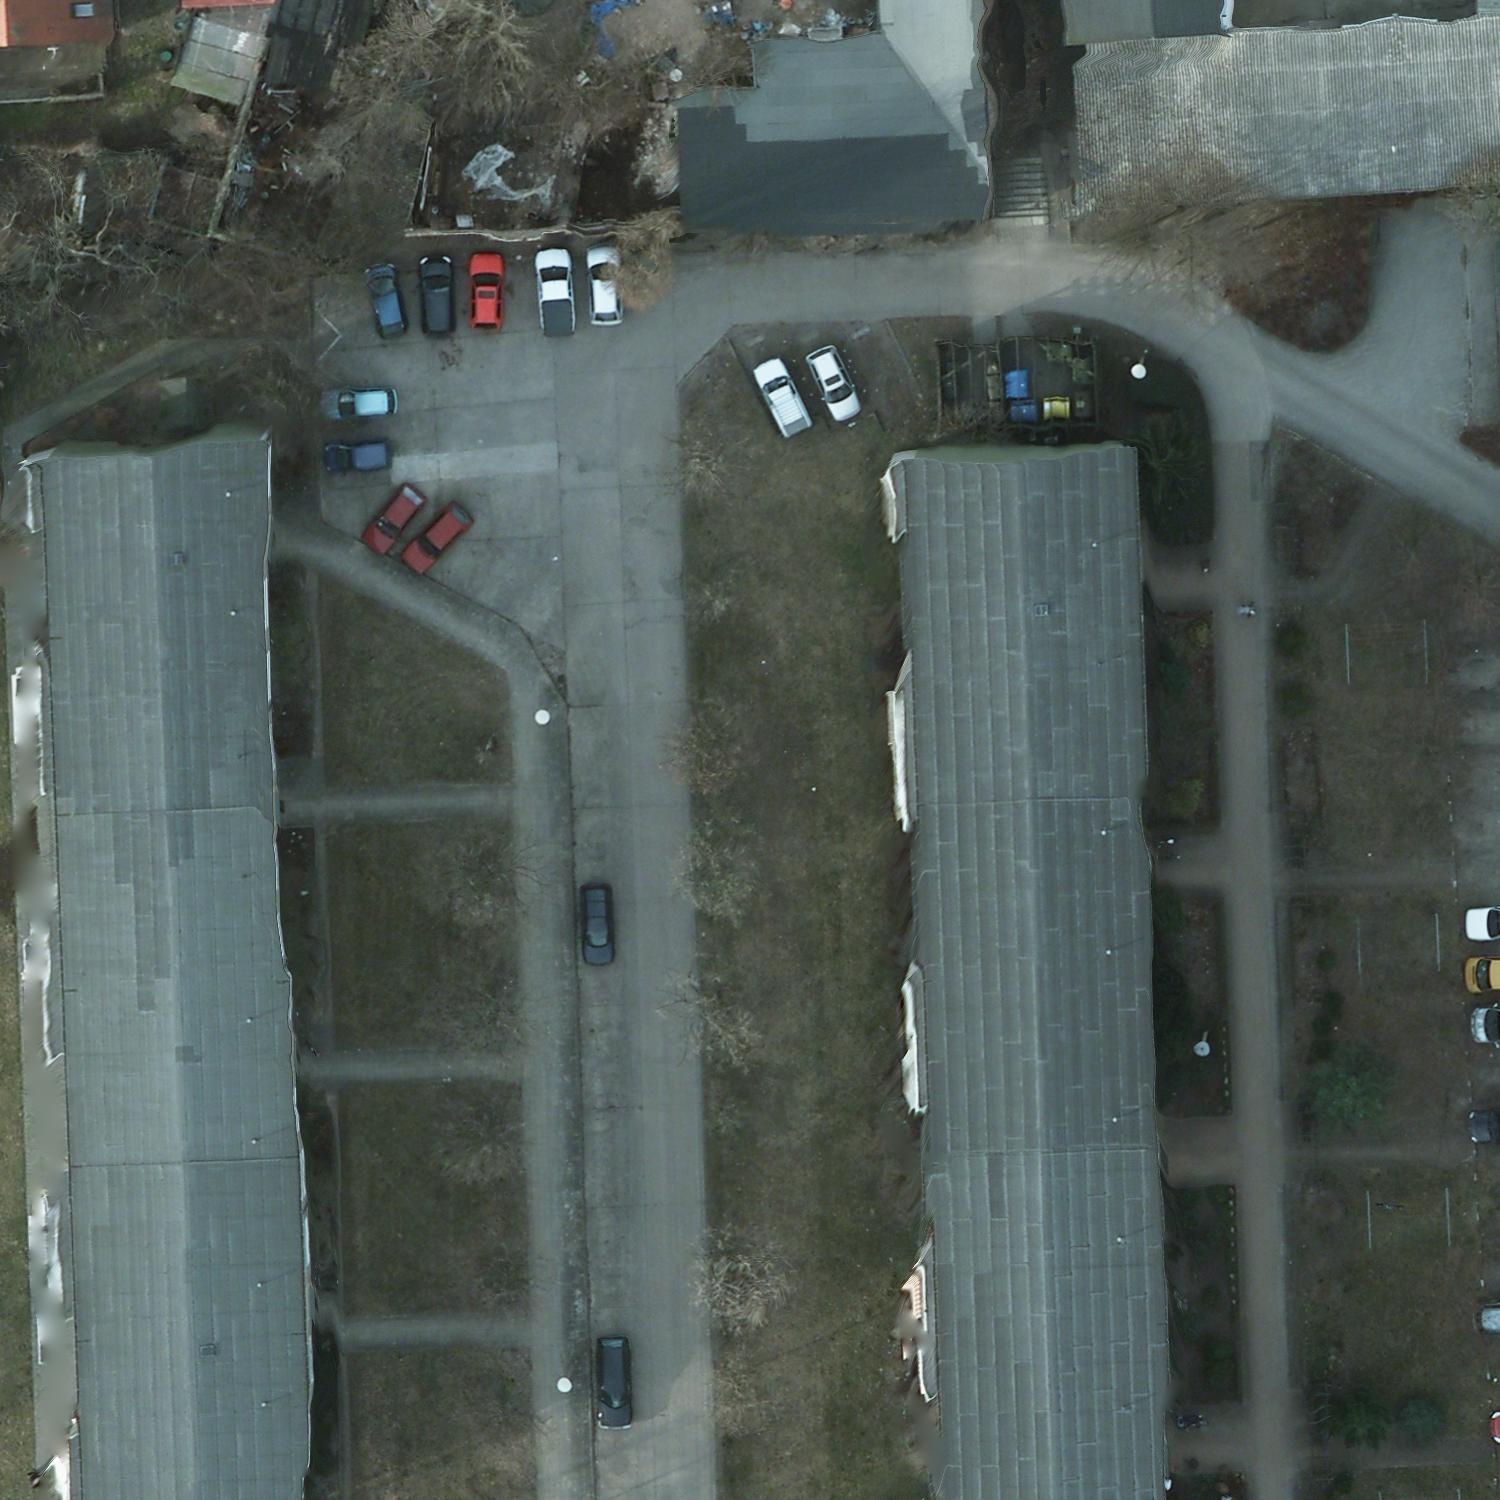
\includegraphics[width=\textwidth]{Chapitre2/potsdam}
    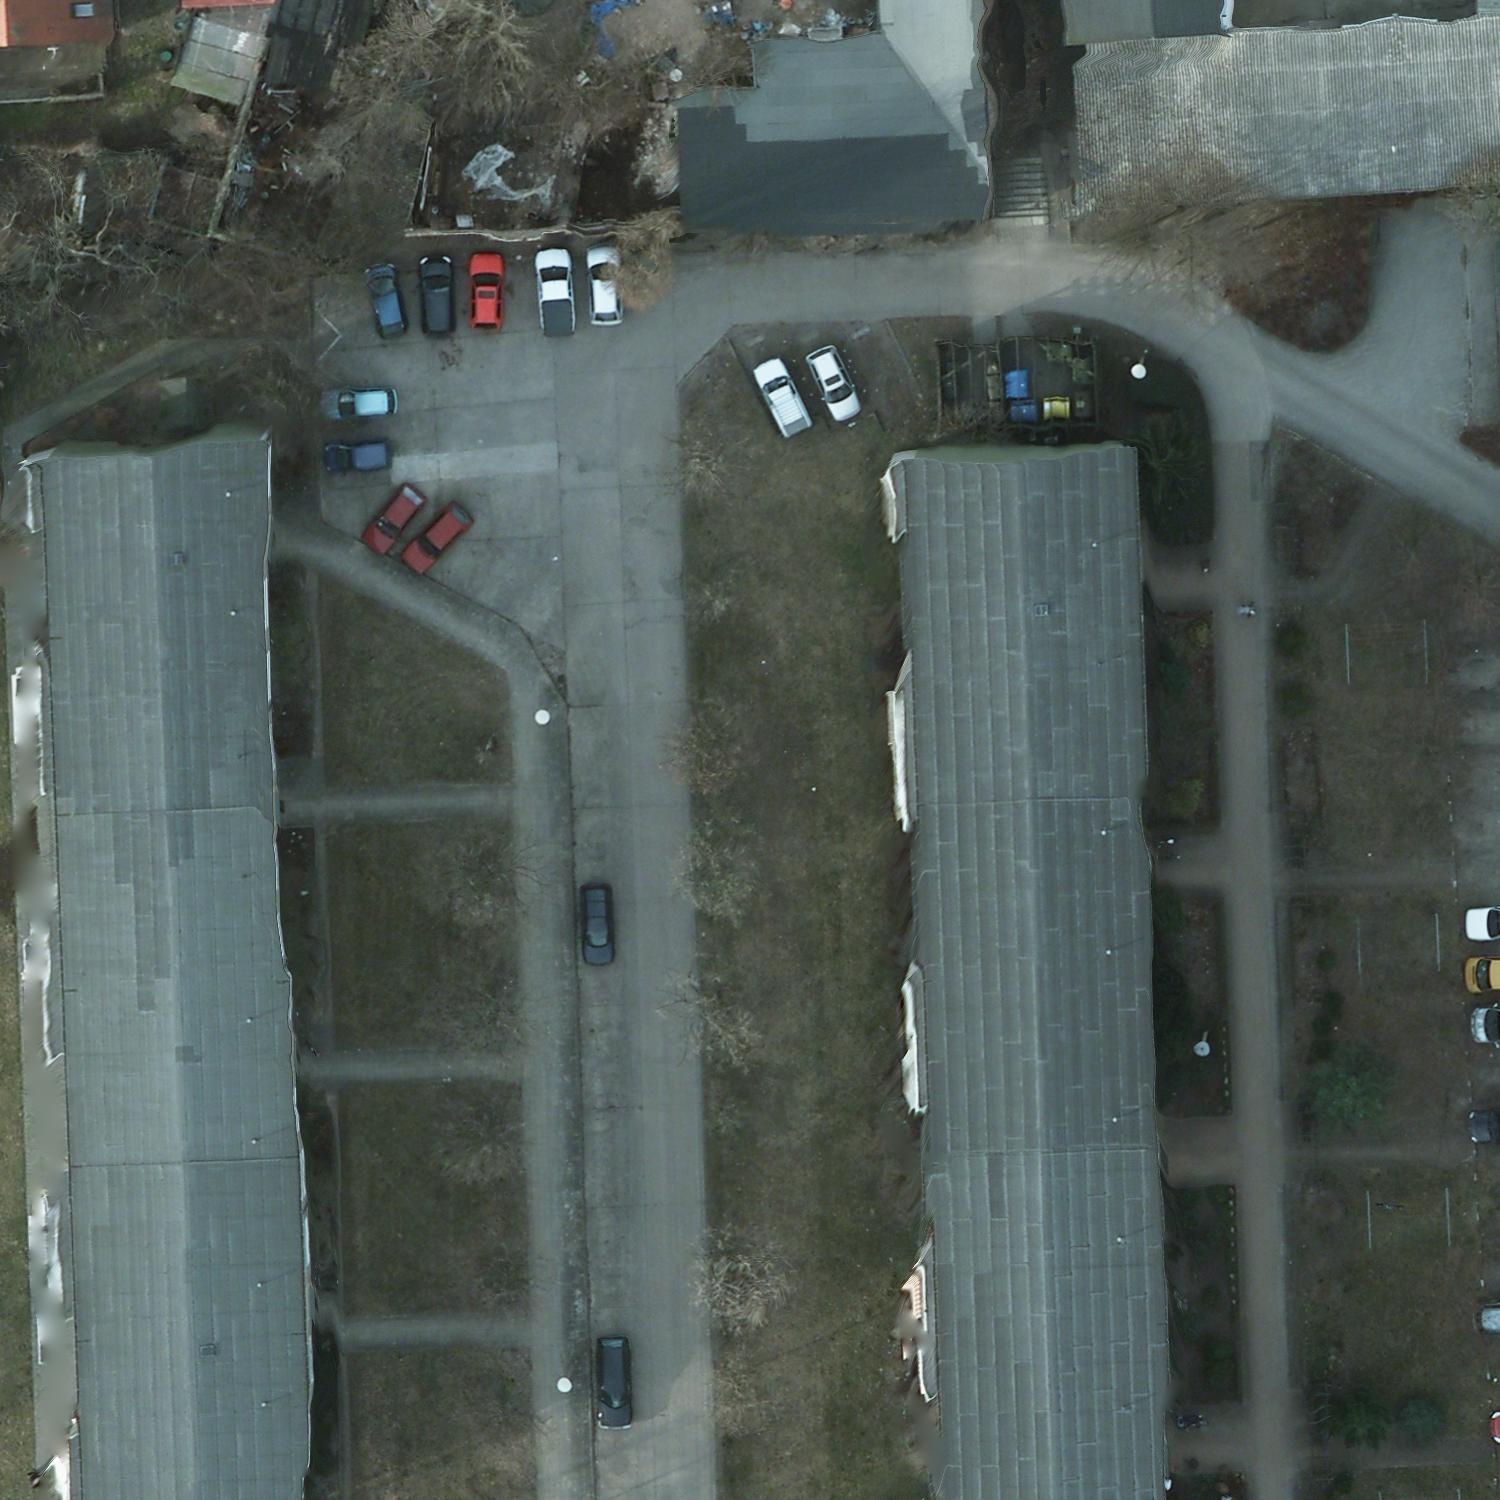
\includegraphics[width=\textwidth]{Chapitre2/potsdam}
    \caption*{Image originale}
\end{subfigure}%
\begin{subfigure}{0.25\textwidth}
    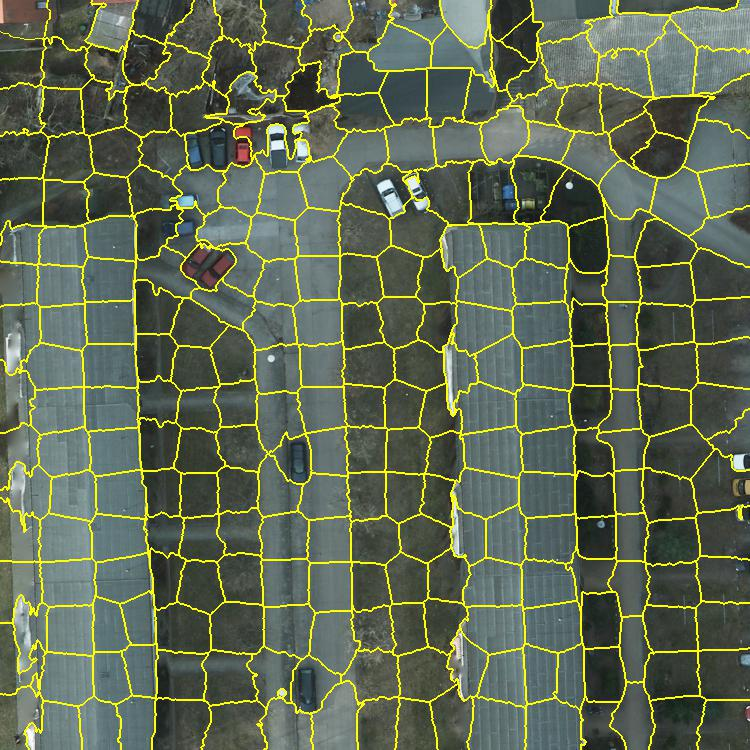
\includegraphics[width=\textwidth]{Chapitre2/potsdam_slic}
    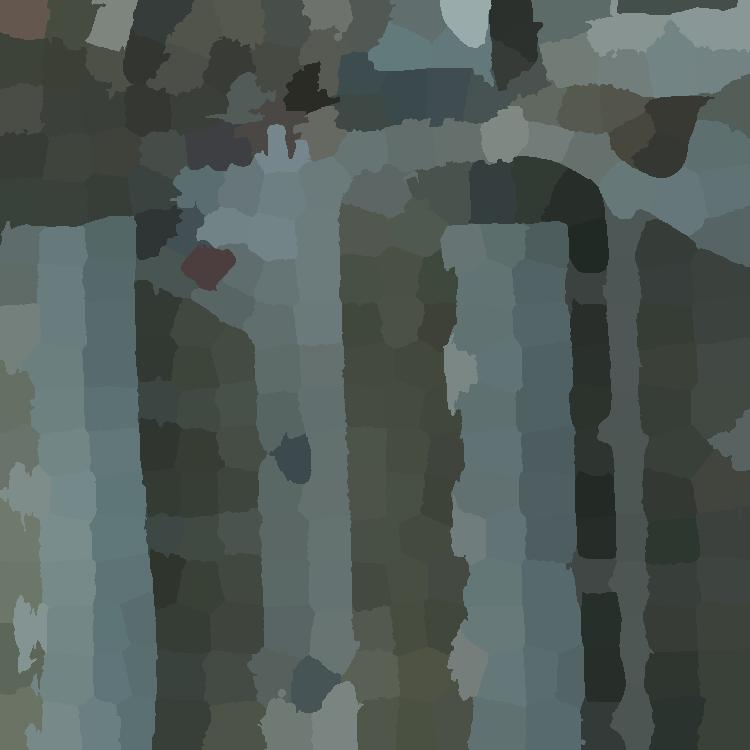
\includegraphics[width=\textwidth]{Chapitre2/potsdam_slic_patchwork}
    \caption*{SLIC}
\end{subfigure}%
\begin{subfigure}{0.25\textwidth}
    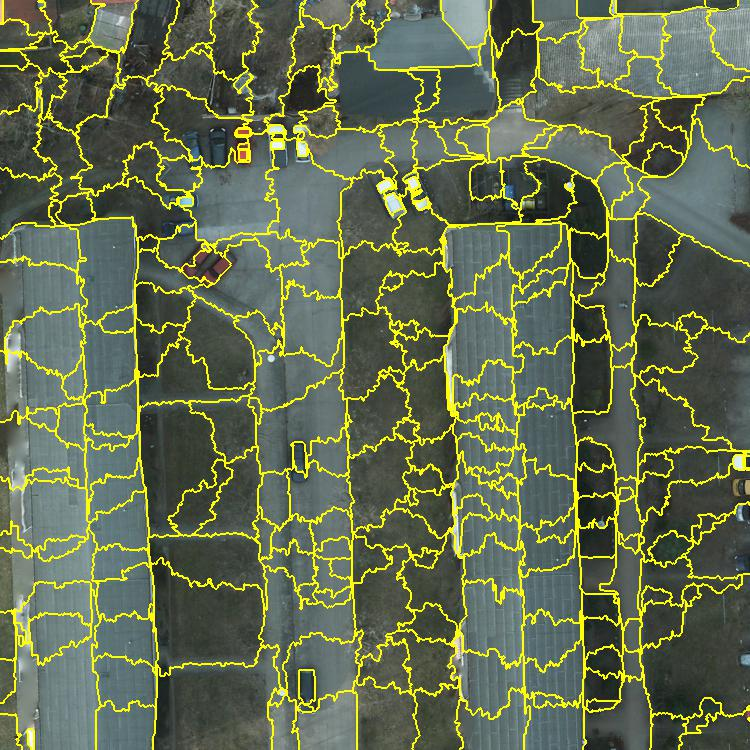
\includegraphics[width=\textwidth]{Chapitre2/potsdam_quickshift}
    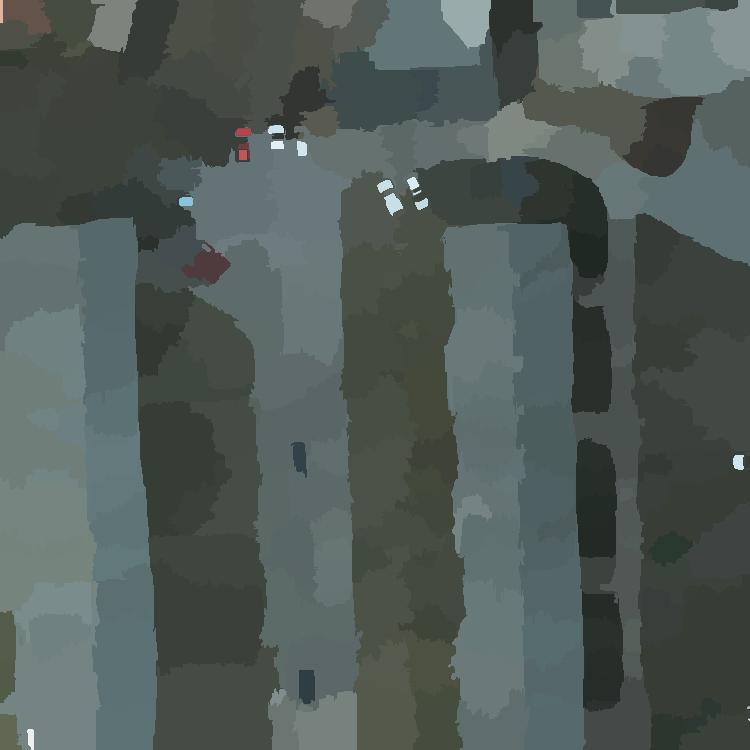
\includegraphics[width=\textwidth]{Chapitre2/potsdam_quickshift_patchwork}
    \caption*{Quickshift}
\end{subfigure}%
\begin{subfigure}{0.25\textwidth}
    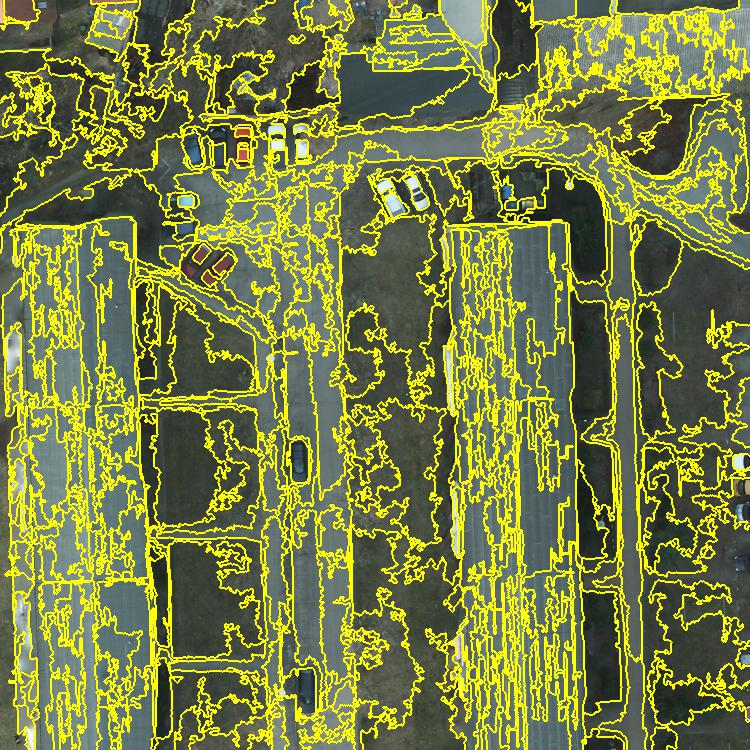
\includegraphics[width=\textwidth]{Chapitre2/potsdam_ecognition}
    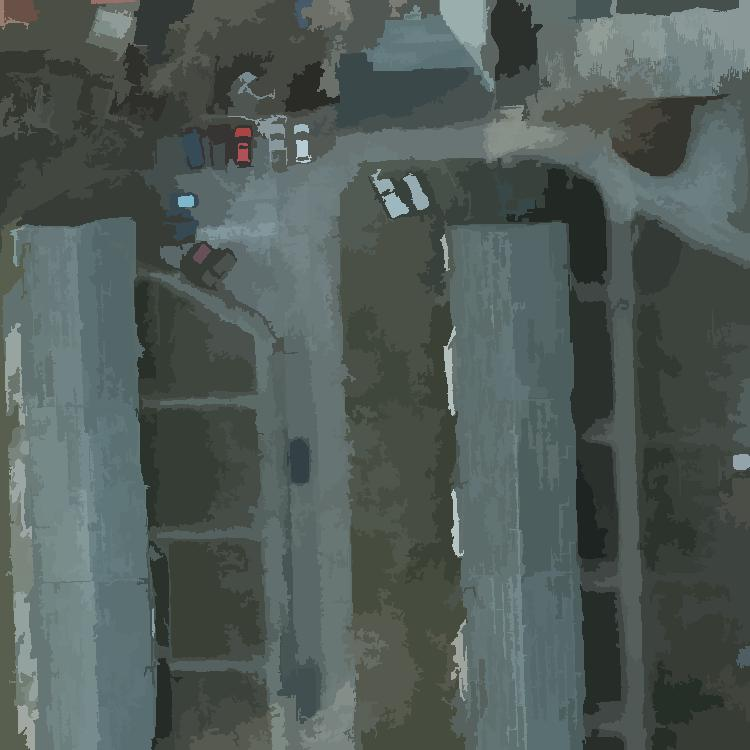
\includegraphics[width=\textwidth]{Chapitre2/potsdam_ecognition_patchwork}
    \caption*{Algorithme MRS}
\end{subfigure}
\caption{Segmentations d'une image aérienne. Selon l'algorithme appliqué, les voitures sont plus ou moins bien segmentées.}
\label{fig:potsdam_segmentation}
\end{subfigure}

\caption{Exemples de segmentation sur deux types d'images. Bien que chaque méthode produise approximativement le même nombre de régions, les détails peuvent parfois être absorbées dans des régions plus grandes.}
\label{fig:segmentation}
\end{figure}

Il existe aussi des segmentations hiérarchiques "HSEG" etc. qui permettent d'extraire des attributs multi-échelles naturellement.

Ensuite, on peut extraire des attributs sur ces régions et classer l'image région par région.

L'avantage principal de ces méthodes est de grandement réduire la complexité calculatoire. Notamment, lorsque l'image augmente de résolution spatiale, de nombreuses régions conservent leur homogénéité et il est ainsi très avantageux de les conserver regroupées.

On peut noter que traiter l'image par une fenêtre glissante ou même par une grille de pixels correspond à des cas particuliers de classification par région.

\subsection{Extraction de caractéristiques}

Données brutes : valeur des intensités lumineuses, radiométrie dans le cas multispectral
  => Problèmes d'amplitude, normalisation, faible robustesse au bruit

Statistiques (min, max, moyenne, médiane, variance) : valeurs annexes
  => choix des indicateurs ?

Indices : NDVI, NDWI
  => choix des indicateurs ?

Histogrammes de couleur : représente la distribution de l'intensité
  => Discrétisation, perte de la spatialisation

Histogrammes de gradient : représente les variations locales avec direction
  => paramètres du gradient à calculer ?

Caractéristiques : peuvent être multi-échelle (différentes tailles de contexte spatial) et multi-sources (différentes données d'entrée)

\subsection{Modèles statistiques usuels}

Arbre de décision : par ensemble = forêt aléatoire

SVM : dans le cas de grandes tailles, optimisation par descente de gradient

XGBoost : gradient boosting d'arbres

\section{Réseaux de neurones profonds}

\subsection{Réseaux de neurones artificiels}

Inspiré de la biologie

Neurone = fonction de transfert non-linéaire

Combinaison de neurones : un neurone est lié par des synapses à d'autres, avec un poids
$\rightarrow$ graphe orienté pondéré

Théorème d'approximation universelle

Rétropropagation

Nombre de couches, nombre de neurones

Régularisation (dropout, pénalité sur les poids)

\subsection{Réseaux de neurones artificiels convolutifs}

Enchaînement de convolutions + activations non linéaires

Partie finale entièrement connectée : classifieur

L'extraction des caractéristiques et la classification se font de manière conjointe : optimisation de bout en bout

\subsection{Réseaux de neurones entièrement convolutifs}

On enlève la partie entièrement connectée pour en faire une partie convolutive

Avantage : prédiction spatiale et non plus unidimensionnelle
Avantage : plus de taille fixée d'image
Avantage : on fait automatiquement la classification pixellique !

\subsection{Application à la cartographie sémantique}

Transposition de SegNet et autres aux images aériennes : pas de verrou particulier

Fenêtre glissante, traitement par batchs, random sampling, augmentation de données

\section{Évaluation des modèles}

Scores F1, précision, rappel, taux de bonne classification, intersection sur union

\section{Bases de données}

\subsection{ISPRS 2D Semantic Labeling}

\subsection{ONERA Christchurch}

\subsection{Data Fusion Contest 2015}

\subsection{Inria Aerial Image Labeling}
	
\bibliographystyle{francaissc}
\bibliography{Chapitre2/Biblio}
